\documentclass[a4paper]{article}
%\usepackage{mathptmx}
\usepackage{amsmath}
\usepackage{amssymb}
\usepackage{amsthm}
\usepackage[retainorgcmds]{IEEEtrantools}
%\usepackage[square]{natbib}

% needs debian package texlive-math-extra
\usepackage{stmaryrd} % for \llbracket, \rrbracket (scott brackets)

\usepackage{tikz}
\usetikzlibrary{positioning}
\usetikzlibrary{matrix}

\newcommand{\arr}{\rightarrow}
\newcommand{\todo}[1]{\bigskip \noindent \emph{todo: #1}}
%\newcommand{\todo}[1]{}
\newcommand{\semantics}[1]{\llbracket #1 \rrbracket}

\newtheorem{defNuF}{Definition}[section]
\newtheorem{defNplaceSeparatedSum}[defNuF]{Definition}
\newtheorem{defF}[defNuF]{Definition}
\newtheorem{thmDomNuFisFixedPoint}[defNuF]{Proposition}
\newtheorem{defNuFCoalgebra}[defNuF]{Definition}
\newtheorem{obsNuFCoalgebraIsInjective}[defNuF]{Observation}
\newtheorem{defNuFCoalgebraPrime}[defNuF]{Definition}
\newtheorem{thmDomNuFisFinal}[defNuF]{Proposition}
\newtheorem{defSemantics}[defNuF]{Definition}
\newtheorem{lemSemanticAfterDeltaIsIdentity}[defNuF]{Lemma}
\newtheorem{lemSemanticAndFagreeOnOneStep}[defNuF]{Lemma}
\newtheorem{defStrictOrderNuF}[defNuF]{Definition}
\newtheorem{defPartialOrderNuF}[defNuF]{Definition}
\newtheorem{thmPONuFisPartialOrder}[defNuF]{Proposition}
\newtheorem{thmPONuFisChainComplete}[defNuF]{Proposition}
\newtheorem{thmPONuFisADomain}[defNuF]{Proposition}
\newtheorem{defPMapsNuFToL}[defNuF]{Definition}
\newtheorem{thmPIsMonotone}[defNuF]{Proposition}
\newtheorem{thmPIsContinuous}[defNuF]{Proposition}

\begin{document}

\title{A Domain For The Natural Numbers With Computation Steps}
\author{Markus Klinik}
\maketitle

%\begin{abstract}
%Lorem ipsum.
%\end{abstract}

\section{What Are The Natural Numbers With Computation Steps?}

\section{What Is a Domain?}

\begin{itemize}

\item A domain is a CPO with a least element.

\item And what is a CPO?  A partial order where every chain has a least upper bound.

\item Finding a domain for the 1+X+X means finding a suitable CPO
together with a mapping from the 1+X+X to that CPO.

\item We then need to prove that the given construction is indeed a CPO with
least element.

\end{itemize}

\section{A Domain for 1+X+X}

\todo{We are currently on vacation in the land of CPOs and strict maps between them.
Or somesuch.}

\begin{defNplaceSeparatedSum}

The I-place separated sum functor is defined as follows.

\begin{equation}
\sum : \mathbf{Cpo}^I \arr \mathbf{Cpo} \nonumber
\end{equation}

\begin{equation}
\sum_{i \in I}{X_i} =
  \bigcup_{i \in I} \{ \langle i, a \rangle | a \in X_i \}
  \cup \{ \bot \} \nonumber
\end{equation}

\begin{equation}
\sum_{i \in I}{(f_i : X_i \arr Y_i)} :
  \sum_{i \in I}{X_i} \arr \sum_{i \in I}{Y_i} \nonumber
\end{equation}

\begin{equation*}
( \sum_{i \in I}f_i ) (x) = \left\{
  \begin{array}{rl}
     \langle i, f(a) \rangle & \text{if } x = \langle i, a \rangle
                               \text{ for some } i \in I \\
    \bot                     & \text{if } x = \bot
  \end{array} \right.
\end{equation*}

\end{defNplaceSeparatedSum}

That is, $\Sigma$ takes a family of sets to their disjoint union and adds a bottom
element to the result.  For a family of functions, it applies the corresponding
function to an element of the disjoint union.  We write $\kappa_i(a)$ for
$\langle i, a \rangle$.

\begin{defF}

The functor F is then defined as follows.

\begin{equation*}
FX = \sum{(1, X, X)}
\end{equation*}

\begin{equation*}
F(f : X \arr Y) = \sum{(\text{id}, f, f)}
\end{equation*}

Where $1 = \{*\}$ is the singleton CPO.

\end{defF}


\begin{defNuF}

Let $Z$ be the set of finite and infinite words generated by the following
grammar.

\begin{equation*}
Z ::= 0 \ |\ \bot \ |\ S Z \ |\ \_ Z
\end{equation*}

\end{defNuF}

Among those words are, for example, all Peano numbers like $0$, $S0$, $SS0$.
We also have arbitrary underscores mixed in between the successors: $\_0$,
$S\_S\_0$.  Instead of $0$, words can be terminated by $\bot$, e.g.  $S\bot$,
$S\_S\bot$.

Note that all finite words are finite sequences of $S$ and $\_$ which end with
either $0$ or $\bot$. All infinite words are $\omega$-sequences of $S$ and $\_$.

We write $|w|$ to denote the length of a word $w$.  The concatenation of two
words $w$, $v$ is denoted by their juxtaposition $wv$.  If $w$ or $v$ are
singleton words, we regard them sometimes as letters, sometimes as words, as the
situation requires.  If $w$ is of length at least $n+1$ then $w_n$ denotes the
$n$th letter of $w$.

\begin{thmDomNuFisFixedPoint}

The set $Z$ is a fixed point of the functor $F$.

\end{thmDomNuFisFixedPoint}

\begin{proof}

We need to show that $Z$ is isomorphic to $FZ$, that is, provide two functions
$\delta : Z \arr FZ$ and $\delta' : FZ \arr Z$ such that their composition is
the identity function, i.e.~$\delta \circ \delta' = \text{id}_{FZ}$ and $\delta'
\circ \delta = \text{id}_Z$.

\begin{defNuFCoalgebra}
Let $\delta : Z \arr FZ$ be defined as
  \begin{IEEEeqnarray}{rCl}
  \delta(\bot) & = & \bot \nonumber
  \\
  \delta(0) & = & \kappa_0(*) \nonumber
  \\
  \delta(Sw) & = & \kappa_1(w) \text{, for all } w \in Z  \nonumber
  \\
  \delta(\_w) & = & \kappa_2(w) \text{, for all } w \in Z  \nonumber
  \end{IEEEeqnarray}
\end{defNuFCoalgebra}

\begin{defNuFCoalgebraPrime}
Let $\delta' : FZ \arr Z$ be defined as
  \begin{IEEEeqnarray}{rCl}
  \delta'(\bot) & = & \bot \nonumber
  \\
  \delta'(\kappa_0(*)) & = & 0 \nonumber
  \\
  \delta'(\kappa_1(w)) & = & Sw \text{, for all } w \in Z  \nonumber
  \\
  \delta'(\kappa_2(w)) & = & \_w \text{, for all } w \in Z  \nonumber
  \end{IEEEeqnarray}
\end{defNuFCoalgebraPrime}

These equations hold.

\begin{IEEEeqnarray}{rCl}
\delta'(\delta(\bot)) & = & \delta'(\bot) = \bot \nonumber
\\
\delta'(\delta(0)) & = & \delta'(\kappa_0(*)) = 0 \nonumber
\\
\delta'(\delta(Sw)) & = & \delta'(\kappa_1(w)) = Sw \text{, for all } w \in Z \nonumber
\\
\delta'(\delta(\_w)) & = & \delta'(\kappa_2(w)) = \_w \text{, for all } w \in Z  \nonumber
\end{IEEEeqnarray}

\begin{IEEEeqnarray}{rCl}
\delta(\delta'(\bot)) & = & \delta(\bot) = \bot \nonumber
\\
\delta(\delta'(\kappa_0(*))) & = & \delta(0) = \kappa_0(*) \nonumber
\\
\delta(\delta'(\kappa_1(w))) & = & \delta(Sw)) = \kappa_1(w) \text{, for all } w \in Z  \nonumber
\\
\delta(\delta'(\kappa_2(w))) & = & \delta(\_w) = \kappa_2(w) \text{, for all } w \in Z  \nonumber
\end{IEEEeqnarray}

\end{proof}

\begin{obsNuFCoalgebraIsInjective}
$\delta$ is injective. \qed
\end{obsNuFCoalgebraIsInjective}

\begin{thmDomNuFisFinal}
\label{thmDomNuFisFinal}

The set $Z$ is the largest fixed point for the functor $F$.

\end{thmDomNuFisFinal}

We need to show that any other fixed point of $F$ can be embedded into $Z$.  We
prove this by showing that $(Z, \delta)$ is a final coalgebra for $F$, that is,
for any other $F$-coalgebra $(C, \gamma : C \arr FC)$ there exists a unique
function $\semantics{-}_{\gamma} : C \arr Z$ such that
$F(\semantics{-}_{\gamma}) \circ \gamma = \delta \circ \semantics{-}_{\gamma}$,
i.e.~it makes the following diagram commute.

\begin{figure}[h]
\begin{center}
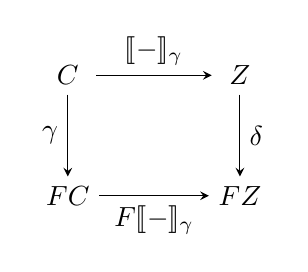
\begin{tikzpicture}
\matrix (m) [matrix of math nodes,row sep=3em,column sep=4em,minimum width=2em]
  {
     C & Z \\
     FC & FZ \\
  };
  \path[-stealth]
    (m-1-1) edge node [left] {$\gamma$} (m-2-1)
            edge node [above] {$\semantics{-}_{\gamma}$} (m-1-2)
    (m-2-1.east|-m-2-2) edge node [below] {$F\semantics{-}_{\gamma}$} (m-2-2)
    (m-1-2) edge node [right] {$\delta$} (m-2-2);
\end{tikzpicture}
\end{center}
\end{figure}

Before we prove this proposition, let's briefly reflect on what it would mean
for $(Z, \delta)$ to be the final coalgebra for $F$.

The idea behind the definitions of $Z$ and $\delta$ is that $Z$ has intrinsic
structure which resembles the structure of $F$.  We can regard $F$-coalgebras as
calculations that either diverge, terminate, or make one of two different
computation steps.  This is encoded as $\gamma(a)$ yielding $\bot$,
$\kappa_0(*)$, $\kappa_1(b)$ or $\kappa_2(b)$ respectively, where $a$ and $b$
are elements of $C$, which we regard as internal states of the computation. In
the latter two cases, the computation can continue from $b$, yielding another
one of the possible outcomes in the next step.

The set $Z$ has as elements finite and infinite words, where we can see one word
as the complete encoding of the behaviour of some $F$-coalgebra.  For example,
take $C = \{\bot, a\}$ and $\gamma(a) = \kappa_0(*)$, then the coalgebra $(C,
\gamma)$, has a very simple behaviour on $a$:  It terminates in the first step.
This behaviour is encoded in the singleton word $0$ in $Z$.

For another example, consider $C$ as above, but this time $\gamma(a) =
\kappa_1(a)$, i.e.~the computation makes one step and yields the state $a$
again.  From there, it continues with the same step, and so on, indefinitely.
This behaviour is represented in $Z$ by the infinite word of only Ss.

The function $\delta$ strips off the first letter of a word $w$, if possible,
and yields as result the rest of the word.  This corresponds to the behaviour of
$\gamma$ on some state $x$: $\gamma$ makes one step, and leaves us with the rest
of it's behaviour.  Our goal is to map $x$ to $w$ such that $\delta$ and
$\gamma$ coincide.

The intrinsic structure of $Z$ makes it possible to embed the states of other
$F$-coalgebras into $Z$. We map a state to the word which corresponds to the
state's behaviour.

\begin{defSemantics}

Let $(C, \gamma)$ be an $F$-coalgebra.  The function $\semantics{-}_{\gamma} : C
\arr Z$ is defined as follows.
\begin{IEEEeqnarray}{rCl}
\semantics{a}_{\gamma} & = & \text{ case } \gamma(a) \text{ of} \nonumber
\\
\bot_C & = & \bot_Z \nonumber
\\
\kappa_0(*) & = & 0 \nonumber
\\
\kappa_1(b) & = & S \semantics{b}_{\gamma} \nonumber
\\
\kappa_2(b) & = & \_ \semantics{b}_{\gamma} \nonumber
\end{IEEEeqnarray}

\end{defSemantics}

If it is clear from the context, we omit the subscript in
$\semantics{-}_{\gamma}$ and write $\semantics{-}$.


\begin{lemSemanticAfterDeltaIsIdentity}
\label{lemSemanticAfterDeltaIsIdentity}

$\semantics{-}_{F\delta} \circ \delta = \text{id}_{Z}$

\end{lemSemanticAfterDeltaIsIdentity}

\newcommand{\semanticsFd}[1]{\semantics{#1}_{F\delta}}

\begin{proof}

By induction on the length of $w \in Z$.

Case $w = \bot$:
\begin{equation*}
\semanticsFd{\delta(\bot)}
  = \semanticsFd{\bot}
  = \bot
\end{equation*}

Case $w = 0$:
\begin{equation*}
\semanticsFd{\delta(0)}
  = \semanticsFd{\kappa_0(*)}
  = \text{case } F\delta(\kappa_0(*)) \text{ of } \ldots
  = \text{case } \kappa_0(\text{id}(*)) \text{ of } \ldots
  = 0
\end{equation*}

Case $w = Sw'$:
\begin{IEEEeqnarray*}{r.l}
   & \semanticsFd{\delta(Sw')} \\
 = & \text{(definition of $\delta$)} \\
   & \semanticsFd{\kappa_1(w')} \\
 = & \text{(definition of $\semantics{-}$)} \\
   & \text{case } F\delta(\kappa_1(w')) \text{ of } \ldots \\
 = & \text{(definition of $F$)} \\
   & \text{case } \kappa_1(\delta(w')) \text{ of } \ldots \\
 = & \text{(definition of $\semantics{-}$)} \\
   & S\semanticsFd{\delta(w')} \\
 = & \text{(induction hypothesis)} \\
   & Sw'
\end{IEEEeqnarray*}

Case $w = \_w'$: Similar to the case $w = Sw'$ but with $\kappa_2$ instead of
$\kappa_1$.

\end{proof}


\begin{lemSemanticAndFagreeOnOneStep}
\label{lemSemanticAndFagreeOnOneStep}

Let $(C, \gamma)$ be an $F$-coalgebra. For any $F$-coalgebra homomorphism $f : C
\arr Z$, all $a$ in $C$ and $w$ in $\{S, \_\}^*$:

\begin{enumerate}

\item
  If $\gamma(a) = \bot$ then $\delta(wf(a)) = \delta(w\bot)$.
\item
  If $\gamma(a) = \kappa_0(*)$ then $\delta(wf(a)) = \delta(w0)$.
\item
  If $\gamma(a) = \kappa_1(b)$ then $\delta(wf(a)) = \delta(wSf(b))$.
\item
  If $\gamma(a) = \kappa_2(b)$ then $\delta(wf(a)) = \delta(w\_f(b))$.

\end{enumerate}

\end{lemSemanticAndFagreeOnOneStep}

\begin{proof}

\begin{enumerate}

% \gamma(a) = \bot
\item
By induction on the length of $w$.

Case $w = \varepsilon$:
\begin{IEEEeqnarray*}{r.l}
    & \delta(f(a)) \\
  = & \text{($f$ is a homomorphism)} \\
    & Ff(\gamma(a)) \\
  = & \text{(assumption)} \\
    & Ff(\bot) \\
  = & \text{(definition of $F$)} \\
    & \bot \\
  = & \text{(definition of $\delta$)} \\
    & \delta(\bot)
\end{IEEEeqnarray*}

Case $w = Sw'$:
\begin{IEEEeqnarray*}{r.l}
    & \delta(Sw'f(a)) \\
  = & \text{(definition of $\delta$)} \\
    & \kappa_1(w'f(a)) \\
  = & \text{(Lemma \ref{lemSemanticAfterDeltaIsIdentity})} \\
    & \kappa_1(\semanticsFd{\delta(w'f(a))}) \\
  = & \text{(induction hypothesis)} \\
    & \kappa_1(\semanticsFd{\delta(w'0)}) \\
  = & \text{(Lemma \ref{lemSemanticAfterDeltaIsIdentity})} \\
    & \kappa_1(w'0) \\
  = & \text{(definition of $\delta$)} \\
    & \delta(Sw'0) \\
  = & \delta(w0)
\end{IEEEeqnarray*}

Case $w = \_w'$:
Similar to the case $w = Sw'$ but with $\kappa_2$ instead of $\kappa_1$.

% \gamma(a) = \kappa_0
\item
By induction on the length of $w$.  The steps are the same as above, only the
base case now produces a 0.

Case $w = \varepsilon$:
\begin{equation*}
  \delta(f(a)) = Ff(\gamma(a)) = Ff(\kappa_0(*)) = \kappa_0(*) = \delta(0)
\end{equation*}

Case $w = Sw'$:
\begin{IEEEeqnarray*}{r.l}
  \delta(Sw'f(a)) & = \kappa_1(w'f(a)) = \kappa_1(\semanticsFd{\delta(w'f(a))}) \\
  & = \kappa_1(\semanticsFd{\delta(w'0)}) = \kappa_1(w'0) \\
  & = \delta(Sw'0)
\end{IEEEeqnarray*}

Case $w = \_w'$:
Similar to the case $w = Sw'$ but with $\kappa_2$ instead of $\kappa_1$.

% \gamma(a) = \kappa_1
\item
By induction on the length of $w$.  Again, the steps are the same, but with
a different base case.

Case $w = \varepsilon$:
\begin{IEEEeqnarray*}{r.l}
    \delta(f(a))
  = Ff(\gamma(a))
  = Ff(\kappa_1(b))
  = \kappa_1(f(b))
  = \delta(Sf(b))
\end{IEEEeqnarray*}

Case $w = Sw'$:
\begin{IEEEeqnarray*}{r.l}
    \delta(Sw'f(a)) = &
    \kappa_1(w'f(a)) =
    \kappa_1(\semanticsFd{\delta(w'f(a))}) \\
  = & \kappa_1(\semanticsFd{\delta(w'Sf(b))}) \\
  = & \kappa_1(w'Sf(b))
  = \delta(Sw'Sf(b)) \\
  = & \delta(wSf(b))
\end{IEEEeqnarray*}

Case $w = \_w'$:
Similar to the case $w = Sw'$ but with $\kappa_2$ instead of $\kappa_1$.

% \gamma(a) = \kappa_2
\item
Similar to the case $\gamma(a) = \kappa_1(b)$, but now the base case produces an
underscore instead of an $S$.

\end{enumerate}

\end{proof}


The informal idea that $(Z, \delta)$ encodes all possible behaviours of
$F$-coalgebras is made explicit in the following proof of proposition
\ref{thmDomNuFisFinal}.

\begin{proof}{(Proposition \ref{thmDomNuFisFinal})}

We need to prove two things.

  \begin{enumerate}
  \item
    The function $\semantics{-}$ is an $F$-coalgebra homomorphism.
  \item
    The function $\semantics{-}$ is unique, i.e.~any other $F$-coalgebra
    homomorphism $f : C \arr Z$ agrees with $\semantics{-}$ on every element of C.
  \end{enumerate}

1. For $\semantics{-}$ to be an
$F$-coalgebra homomorphism, it has to satisfy the equation $\delta \circ
\semantics{-} = F\semantics{-} \circ \gamma$.  Let $a$ be an element of $C$. We
proceed by case distinction on $\gamma(a)$.

Case $\gamma(a) = \bot$:
\begin{equation*}
\delta(\semantics{a}) = \delta(\bot) = \bot =
F\semantics{\bot} = F\semantics{\gamma(a)}
\end{equation*}

Case $\gamma(a) = \kappa_0(*)$:
\begin{equation*}
\delta(\semantics{a}) = \delta(0) = \kappa_0(*)
= \kappa_0(\text{id}(*)) = F\semantics{\kappa_0(*)} = F\semantics{\gamma(a)}
\end{equation*}

Case $\gamma(a) = \kappa_1(b)$:
\begin{equation*}
\delta(\semantics{a}) = \delta(S \semantics{b}) = \kappa_1(\semantics{b}) =
F\semantics{\kappa_1(b)} = F\semantics{\gamma(a)}
\end{equation*}

Case $\gamma(a) = \kappa_2(b)$:
\begin{equation*}
\delta(\semantics{a}) = \delta(\_ \semantics{b}) = \kappa_2(\semantics{b}) =
F\semantics{\kappa_2(b)} = F\semantics{\gamma(a)}
\end{equation*}

2. For the uniqueness of $\semantics{-}$, assume $f : C \arr Z$ is another
$F$-coalgebra homomorphism, that is, it satisfies the equation $\delta \circ f =
Ff \circ \gamma$.  We proceed by constructing a bisimulation relation between
$\delta \circ f$ and $\delta \circ \semantics{-}$.  Let

\begin{equation*}
R \subseteq FZ \times FZ =
  \{ \langle \delta(wf(a)) , \delta(w\semantics{a}) \rangle
   \ |\  a \in C, w \in \{ S, \_ \}^*
  \}
\end{equation*}

The proof that $R$ is a bisimulation relation goes by case distinction on
$\gamma(a)$.  All cases use the definition of $\semantics{-}$ for the first
equality, and lemma \ref{lemSemanticAndFagreeOnOneStep} for the second one.

Case $\gamma(a) = \bot$:
\begin{IEEEeqnarray*}{C}
  \delta(w\semantics{a}) = \delta(w\bot) = \delta(wf(a))
\end{IEEEeqnarray*}

Case $\gamma(a) = \kappa_0(*)$:
\begin{IEEEeqnarray*}{C}
  \delta(w\semantics{a}) = \delta(w0) = \delta(wf(a))
\end{IEEEeqnarray*}

Case $\gamma(a) = \kappa_1(b)$:
\begin{IEEEeqnarray*}{rCl}
  \delta(w\semantics{a}) & = & \delta(wS\semantics{b}) \\
  \delta(wf(a)) & = & \delta(wSf(b))
\end{IEEEeqnarray*}

Case $\gamma(a) = \kappa_2(b)$:
\begin{IEEEeqnarray*}{rCl}
  \delta(w\semantics{a}) & = & \delta(w\_\semantics{b}) \\
  \delta(wf(a)) & = & \delta(w\_f(b))
\end{IEEEeqnarray*}

In the first two cases, the functions are identical, in the latter two cases,
the functions are again in $R$.  This proves that $R$ is a bisimulation
relation.

For $w = \epsilon$, we have that $\langle \delta(f(a)) , \delta(\semantics{a})
\rangle$ is in $R$ for all $a$ in $C$.  This gives us the equality $\delta \circ
f = \delta \circ \semantics{-}$, from which, by injectivity of $\delta$, we
get $f = \semantics{-}$.


\end{proof}

\begin{defStrictOrderNuF}

Let the relation $\sqsubset$ on $Z \times Z$ be defined as: two
words $s$ and $t$ are in relation $s \sqsubset t$ iff $s$ is finite and $|s|
\leq |t|$ and $s_{|s|-1} = \bot$ and for all $i < |s|-1: s_i = t_i$.

\end{defStrictOrderNuF}


\begin{defPartialOrderNuF}

Let $\sqsubseteq$ be the reflexive closure of $\sqsubset$.

\end{defPartialOrderNuF}


\begin{figure}
\begin{center}
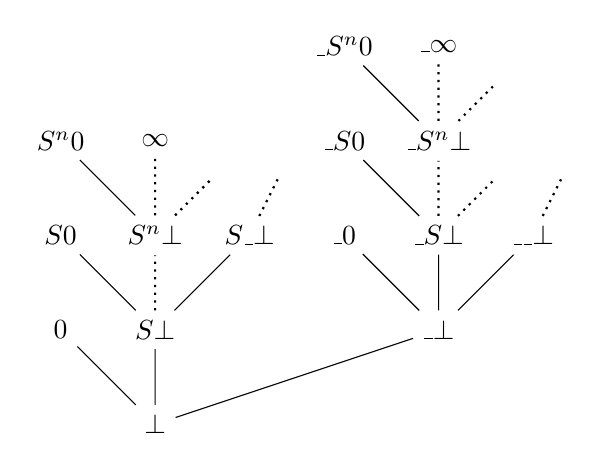
\begin{tikzpicture}
 [ grow'=up
 , scale=1.2
 , level distance=1cm
 , level 1/.style={sibling distance=3cm}
 , level 2/.style={sibling distance=1cm}
 , normal/.style={thin, solid}
 , skipping/.style={thick, dotted}
 , and so on/.style={thick, dotted, sibling distance=0.6cm, level distance=0.6cm}
 ]
  \node {$\bot$}
    child [sibling distance=1cm] { node {$0$} }
    child
    {
      node {$S\bot$}
      child { node {$S0$} }
      child [skipping]
      {
        %node {$SS\bot$}
        %child { node {$SS0$} }
        %child [skipping]
        %{
          node {$S^n\bot$}
          child [normal] { node {$S^n0$} }
          child [skipping] { node {$\infty$} }
          child [and so on] {}
        %}
        %child [and so on] {}
      }
      child
      {
        node {$S\_\bot$}
        child [missing] {}
        child [and so on] {}
      }
    }
    child
    {
      node {$\_ \bot$}
      child { node {$\_0$} }
      child
      {
        node {$\_S\bot$}
        child { node {$\_S0$} }
        child [skipping]
        {
          node {$\_S^n\bot$}
          child [normal] { node {$\_S^n0$} }
          child { node {$\_\infty$} }
          child [and so on] {}
        }
        child [and so on] {}
      }
      child
      {
        node {$\_\_\bot$}
        child [missing] {}
        %child [missing] {}
        child [and so on] {}
      }
    }
  ;
\end{tikzpicture}
\end{center}
\caption{The domain $(Z, \sqsubseteq)$.}
\label{figDomainOfNuF}
\end{figure}

If $s \sqsubseteq t$ we say that $t$ is \emph{above} $s$, or that $s$ is
\emph{below} $t$.  If $s \sqsubset t$ we say $t$ is \emph{strictly above} $s$
and $s$ is \emph{strictly below} $t$.

The definition of $\sqsubseteq$ is intended to define an information ordering on
$Z$.  Its relation graph is shown in figure \ref{figDomainOfNuF}.
Informally speaking, nodes closer to the root of the tree give less information
than nodes further up the tree.  Consider a process that step-by-step calculates
an element of $Z$.  We want to interpret the result of the computation
based on the output we have seen so far.  The root node can then be read as ``it
could be any number''.  The value $S\bot$ can be read as ``it is at least one''.
Any value that ends with a $0$ tells us a concrete number, together with the
fact that the process has terminated.  As with flat domains, concrete values are
incomparable, so we don't distinguish between $1$ and $2$ from the viewpoint of
information ordering.

When looking at the subtree of $\_\bot$, we see that its structure is similar
to the whole domain itself, except that every value is prefixed with one additional
underscore.  Nodes in this subtree can be interpreted similarly as described
above, only that it took the process one internal computation step more to
get to this point.

\begin{thmPONuFisPartialOrder}
\label{thmPONuFisPartialOrder}

The relation $\sqsubseteq$ is a partial order.

\end{thmPONuFisPartialOrder}


\begin{proof}

We have to prove the that $\sqsubseteq$ is reflexive, transitive, and
antisymmetric.

Reflexive: by definition.

Transitive: We have to prove that if $s \sqsubseteq t$ and $t \sqsubseteq u$
then $s \sqsubseteq u$ for all words $s$, $t$, $u$. We do so by distinguishing
four cases.

1. If $s = t = u$ then $s \sqsubseteq u$ follows from reflexivity.

2, 3. The cases $s \neq t \wedge t = u \wedge s \sqsubseteq t$ and $s = t
\wedge t \neq u \wedge t \sqsubseteq u$ are trivial.

4. $s \neq t \wedge t \neq u \wedge s \sqsubseteq t \wedge t \sqsubseteq u$ We
have: $|s| \leq |t| \leq |u|$ and $s_{|s|-1} = \bot$ and $t_{|t|-1} = \bot$ and
for all $i < |s|-1: s_i = t_i$ and for all $j < |t|-1: t_j = u_j$.  But this
means, because of $|s| \leq |t|$: for all $i < |s|-1: s_i = u_i$, hence $s
\sqsubseteq u$.

Antisymmetric: We have to prove that if $s \sqsubseteq t \wedge t \sqsubseteq
s$ then $s = t$.  The premise is either the case because $s = t$ to begin with,
or we have: $s$ is finite and $|s| \leq |t|$ and $s_{|s|-1} = \bot$ and for all $j <
i: s_j = t_j$ and $t$ is finite and $|t| \leq |s|$ and $t_{|t|-1} = \bot$ and for all
$j < i: t_j = s_j$.  But then $s$ and $t$ are both finite, of the same length,
and agree in all elements, hence $s = t$.

\end{proof}

\begin{thmPONuFisChainComplete}
\label{thmPONuFisChainComplete}

The relation $\sqsubseteq$ is chain complete.

\end{thmPONuFisChainComplete}

\begin{proof}

We need to show that every ascending chain in $Z$ has a least upper bound.  An
ascending chain in $Z$ is a sequence $x : \mathbb{N} \arr Z$ such that for all
$i \in \mathbb{N}: x(i) \sqsubseteq x(i + 1)$.

There are two cases.

\begin{enumerate}
  \item
    \label{blahhhh}
    Either the sequence stops growing at some point, i.e.~there is a $j$ such
    that for all $k > j$, $x(j) = x(k)$.
  \item
    The sequence keeps strictly growing, that is, for every $j$ there is a $k$
    such that $k > j$ and $x(j) \sqsubset x(k)$.
\end{enumerate}

In the first case, the element $x(j)$ is the least upper bound of the sequence.

In the second case, we define the infinite word $w$ as follows.  Observe that
all elements $x(j)$ are finite, and consist of a prefix in $\{S, \_\}^*$,
terminated by $\bot$.  This stems from the definition of $\sqsubset$ and the
fact that every $x(j)$ is strictly below some $x(k)$.  The sequence $x$ may
contain repetitions, so we first need to get rid of them. Define the sequence
$x'$ as follows.
\begin{IEEEeqnarray*}{rCl}
x'(0) & = & x(0) \\
x'(n+1) & = & \text{the first } x(j) \text{ such that } x'(n) \sqsubset x(j)
\end{IEEEeqnarray*}
We now take the word $w$ to be the diagonal of $x'$, offset by one, that is,
\begin{equation*}
  w_i = x'(i+1)_i
\end{equation*}
Figure \ref{figExampleXprime} shows an example of such a condensed sequence
$x'$, with the corresponding $w$ highlighted.

\begin{figure}
\begin{center}
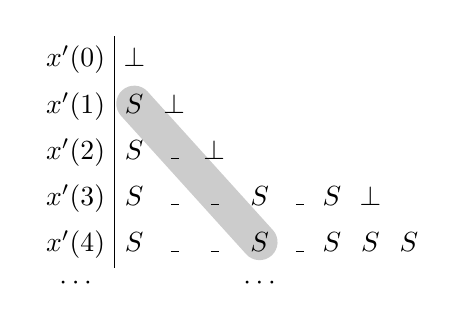
\begin{tikzpicture}
\matrix (m) [matrix of math nodes]
  {
     x'(0) & \bot \\
     x'(1) & S & \bot \\
     x'(2) & S & \_ & \bot \\
     x'(3) & S & \_ & \_ & S & \_ & S & \bot \\
     x'(4) & S & \_ & \_ & S & \_ & S & S & S \\
     \cdots & & & & \cdots \\
  };
  \draw (m-1-1.north east) -- (m-5-1.south east);
  \path (m-2-2.center) -- (m-5-5.center) [draw,line cap=round,line
  width=1.3em,opacity=0.2];
\end{tikzpicture}
\end{center}
\caption{Example of a sequence without repetitions. The first few elements of
$w$ are highlighted.}
\label{figExampleXprime}
\end{figure}

The word $w$ is the least upper bound of the sequence $x$. We have that for
every $i$: $x(i) \sqsubseteq w$, that is, $x(i)$ is finitie, terminated by
$\bot$, and $|x(i)| < |w|$, and $w$ and $x(i)$ agree on all but the last letter
of $x(i)$.

\end{proof}


\begin{thmPONuFisADomain}

The structure $(Z, \sqsubseteq)$ is a domain.

\end{thmPONuFisADomain}

\begin{proof}

We need to show that $(Z, \sqsubseteq)$:

\begin{enumerate}

  \item is a partial order

  \item is chain-complete

  \item has a least element, i.e.~there is an element $s \in Z$ such that for
    any other element $t \in Z, s \sqsubseteq t$.

The first two points have been shown in propositions
\ref{thmPONuFisPartialOrder} and \ref{thmPONuFisChainComplete}.  For the last
point, observe that the word $\bot$ is below any other word.  It is finite, ends
with $\bot$, and the empty word is a prefix of any word.

\end{enumerate}

\end{proof}

Next, we want to check if we can recover the lazy natural numbers, denoted by
$L$ from $Z$ by giving a continuous map between $Z$ and $L$.  The domain $(L,
\sqsubseteq)$ is given informally in figure \ref{figDomainOfLazyNaturals}.

\begin{figure}
\begin{center}
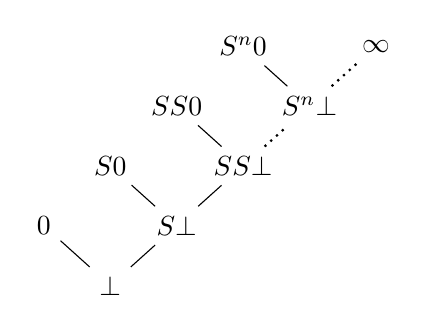
\begin{tikzpicture}[scale=1.2]
  \node {$\bot$} [grow'=up, sibling distance=4.0em, level distance=1.8em]
    child { node {$0$} }
    child
    {
      node {$S\bot$}
      child { node {$S0$} }
      child
      {
        node {$SS\bot$}
        child { node {$SS0$} }
        child [thick, dotted]
        {
          node {$S^n\bot$}
          child [thin, solid] { node {$S^n0$} }
          child { node {$\infty$} }
        }
      }
    }
  ;
\end{tikzpicture}
\end{center}
\caption{The domain of $L$, the lazy natural numbers.}
\label{figDomainOfLazyNaturals}
\end{figure}

\begin{defPMapsNuFToL}

Assuming that we can recognize the word of infinitely many underscores, denoted
by $z$, define the function $p : Z \arr L$ by case distinction on words $w
\in Z$ as follows.

\begin{IEEEeqnarray*}{rCl}
p(\bot) & = & \bot \\
p(z) & = & \bot \\
p(0) & = & 0 \\
p(Sw') & = & Sp(w') \\
p(\_w') & = & p(w')
\end{IEEEeqnarray*}

\end{defPMapsNuFToL}

The function $p$, which projects $Z$ to $L$, discards all underscores which
appear inside words.  If a word ends with the infinite sequence of
underscores, this end part is replaced by $\bot$.  For example, $p(S0) = S0$ and
$p(S\_Sz) = SS\bot$.

From a computational point of view, this means $p$ disregards internal
computation steps, and a process which computes $z$ is equivalent to a diverging
computation.

\begin{thmPIsMonotone}

The function $p$ is monotone.

\end{thmPIsMonotone}

\begin{proof}

We need to prove: for all $s, t \in Z:$ if $s \sqsubseteq t$ then $p(s)
\sqsubseteq p(t)$.  Consider two cases separately:

\begin{enumerate}

  \item
    $s = t$. Because p is a function, $p(s) = p(t)$, hence $p(s) \sqsubseteq
    p(t)$

  \item
    $s \sqsubset t$. We have that $s$ is finite and terminated by $\bot$, and so
    is $p(s)$.  As the initial segments of $s$ and $t$ up to length $|s|-1$
    coincide, so do the initial segments of $p(s)$ and $p(t)$ up to length
    $|p(s)|-1$.  But every word that starts with the same initial segment as
    $p(s)$, no matter how it continues, is above $p(s)$ in $L$, hence $p(s)
    \sqsubseteq p(t)$.

\end{enumerate}

\end{proof}


\begin{thmPIsContinuous}

The function $p$ is continuous.

\end{thmPIsContinuous}

\begin{proof}

Let $x$ be an ascending chain of words in $Z$.  Consider the two cases:

\begin{enumerate}

  \item The chain $x$ stops growing at some point $j \in \mathbb{N}$. Then
  $x(j)$ is the least upper bound of $x$, and by monotonicity of $p$, $p(x(j))$
  is above any $p(x(i))$, $i \in \mathbb{N}$.

  \item Every $x(j)$ is strictly below some other $x(k)$, $j < k$, and $\sqcup
  x$ is the least upper bound of x.  We have that every $x(j)$ is finite and
  ends with $\bot$, so the same holds for every $p(x(j))$.  We also have that
  $\sqcup x$ is an infinite word.  We consider two cases.

    \begin{enumerate}

      \item $\sqcup x$ ends with the word of infinitely many underscores.  That
      is, it has only finitely many $S$s.  This means that after some point $j$,
      all $x(k)$, $k > j$, increase in length but don't get any more $S$s, only
      underscores.  As $p$ discards all underscores, but keeps the final $\bot$,
      all those words get mapped to the same element in $L$, which is the same
      as $p(\sqcup x)$, hence for all $i \in \mathbb{N}$: $p(x(i)) \sqsubseteq
      p(\sqcup x)$.

      \item $\sqcup x$ has infinitely many $S$s.  The projection $p$ maps
      $\sqcup x$ to $\infty \in L$, which is above any word having the shape
      described above.

    \end{enumerate}

\end{enumerate}

\end{proof}

\section{Further directions}

We have given a domain for the functor $FX = \sum{(1, X, X)}$, which makes it
suitable for inclusion in the denotational semantics of programming languages.
One possible further development could be to actually include a data structure
of that type in a suitable programming language, say some coinductive variant of
PCF.  Another, more theoretical, question would be to analyze whether the term
model construction used here could be generalized to arbitrary $F$-coalgebras
where $F$ is a polynomial functor.

\section{Bibliographic notes}

Lorem ipsum \cite{Pierce1991} \cite{Gunter1992} \cite{Bird1997}
\cite{Mitchell1996} \cite{Allison1986} \cite{Capretta2002}

\todo{Barr and Wells "Cats for CompSci", Escardo "On lazy nats"}

\bibliographystyle{plain}
\bibliography{computer_science}
\end{document}

% vim: textwidth=80
